%%%%%%%%%%%%%%%%%%%%%%%%%%%%%%%%%%%%%%%%%%%%%%%%%%%%%%%%%%%%%%%%%%%%%%%%%%%%%%%
% Titel:   Diagramm: SRF02
% Autor:   Nicola Käser
%%%%%%%%%%%%%%%%%%%%%%%%%%%%%%%%%%%%%%%%%%%%%%%%%%%%%%%%%%%%%%%%%%%%%%%%%%%%%%%
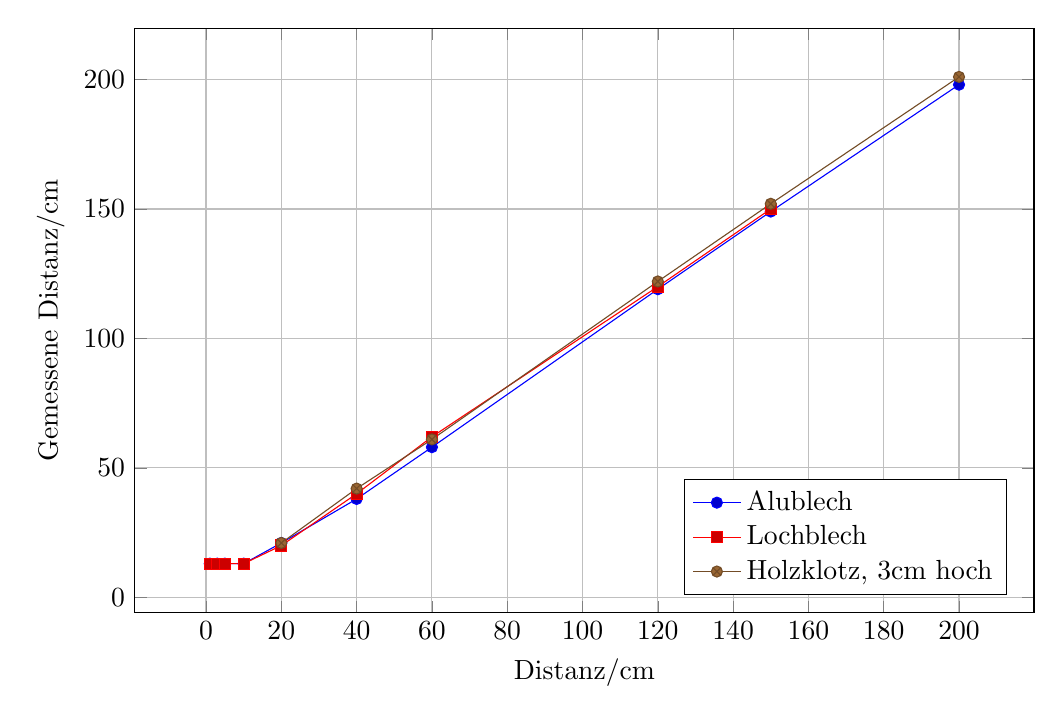
\begin{tikzpicture}
	\begin{axis}[
		height=9cm, width=13cm,
		xlabel=Distanz/cm, ylabel=Gemessene Distanz/cm,
		grid=major,
		legend style={
			cells={anchor=west},
			legend pos=south east
		}]
	%
	%\addplot[color=blue,mark=*] coordinates {
	\addplot coordinates {
		(  1,  13)
		(  3,  13)
		(  5,  13)
		( 10,  13)
		( 20,  21)
		( 40,  38)
		( 60,  58)
		(120, 119)
		(150, 149)
		(200, 198)
	};
	\addlegendentry{Alublech}
	%
	%\addplot[color=red,mark=square*] coordinates {
	\addplot coordinates {
		(  1,  13)
		(  3,  13)
		(  5,  13)
		( 10,  13)
		( 20,  20)
		( 40,  40)
		( 60,  62)
		(120, 120)
		(150, 150)
		%(200, 150)
	};
	\addlegendentry{Lochblech}
	%
	%\addplot[color=teal,mark=triangle*] coordinates {
	\addplot coordinates {
		( 20,  21)
		( 40,  42)
		( 60,  61)
		(120, 122)
		(150, 152)
		(200, 201)
	};
	\addlegendentry{Holzklotz, 3cm hoch}
	%
	\end{axis}
\end{tikzpicture}